\PassOptionsToPackage{table}{xcolor}
\documentclass[12pt,letterpaper,twocolumn,openany,nodeprecatedcode,bg=none]{dndbook}
\usepackage[english]{babel}
\usepackage[utf8]{inputenc}
\usepackage{longtable,booktabs,array}
\usepackage{calc}
\usepackage{etoolbox}
\usepackage{caption}
\usepackage{float}
\usepackage{graphicx}
\usepackage{needspace}
\usepackage{tikz}

% Reset zebra striping at the start of every table
\AtBeginEnvironment{longtable}{\rowcolors{1}{white}{gray!10}\small}
\AtBeginEnvironment{table}{\rowcolors{1}{white}{gray!10}}

\providecommand{\pandocbounded}[1]{#1}
\providecommand{\tightlist}{%
  \setlength{\itemsep}{0pt}\setlength{\parskip}{0pt}}

\captionsetup{labelformat=empty}
\setcounter{secnumdepth}{0}
\setlength{\parindent}{0pt}
\setlength{\parskip}{0.5\baselineskip}
\setlength{\headheight}{15pt}

% Prevent orphaned subsections
\let\oldsubsection\subsection
\renewcommand{\subsection}[1]{%
  \needspace{5\baselineskip}%
  \oldsubsection{#1}%
}

\begin{document}
\onecolumn

      \title{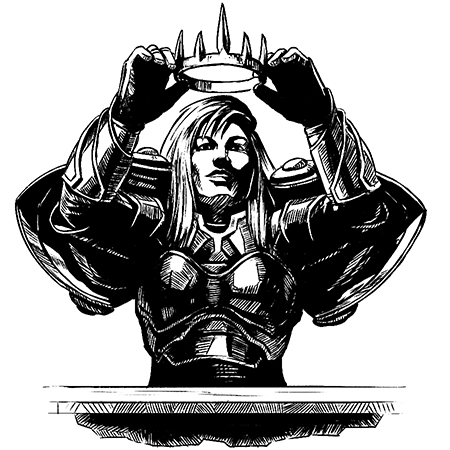
\includegraphics[width=0.9\textwidth,height=0.55\textheight,keepaspectratio]{crownPaladin.jpg}\\[1.5cm]Paladin}
  \author{Class Handbook}
\date{}
\maketitle



\clearpage
\twocolumn

\section{Paladin}\label{paladin}

\subsection{Core Paladin Traits}\label{core-paladin-traits}

\needspace{11\baselineskip}

{\def\LTcaptype{none} % do not increment counter
\begin{table}[!htbp]
\centering
\begin{tabular}{@{}
  >{\raggedright\arraybackslash}p{(\linewidth - 2\tabcolsep) * \real{0.3768}}
  >{\raggedright\arraybackslash}p{(\linewidth - 2\tabcolsep) * \real{0.6232}}@{}}
\toprule\noalign{}
\begin{minipage}[b]{\linewidth}\raggedright
\textbf{Primary Ability}
\end{minipage} & \begin{minipage}[b]{\linewidth}\raggedright
Strength
\end{minipage} \\
\midrule\noalign{}
\textbf{Hit Points} & 1d8 \\
\textbf{Saving Throw Proficiencies} & Strength, Constitution, Wisdom,
Charisma \\
\textbf{Skill Proficiencies} & Choose 2 skills \\
\textbf{Weapon Proficiencies} & Choose 3 categories \\
\textbf{Starting Equipment} & Chain Mail, Longsword, Large Shield,
Dagger \\
\bottomrule\noalign{}
\end{tabular}
\end{table}
}

\subsection{Paladin Features}\label{paladin-features}

\needspace{20\baselineskip}

{\def\LTcaptype{none} % do not increment counter
\begin{table}[!htbp]
\centering
\begin{tabular}{@{}
  >{\raggedright\arraybackslash}p{(\linewidth - 4\tabcolsep) * \real{0.1087}}
  >{\raggedright\arraybackslash}p{(\linewidth - 4\tabcolsep) * \real{0.2391}}
  >{\raggedright\arraybackslash}p{(\linewidth - 4\tabcolsep) * \real{0.6522}}@{}}
\toprule\noalign{}
\begin{minipage}[b]{\linewidth}\raggedright
Level
\end{minipage} & \begin{minipage}[b]{\linewidth}\raggedright
Proficiency
\end{minipage} & \begin{minipage}[b]{\linewidth}\raggedright
Class Features
\end{minipage} \\
\midrule\noalign{}
1 & +2 & Detect Alignment, Divine Aura \\
2 & +2 & --- \\
3 & +2 & Ability Bonus, Turn Undead \\
4 & +2 & --- \\
5 & +2 & Two Attacks \\
6 & +2 & --- \\
7 & +2 & Ability Bonus, Protective Aura \\
8 & +2 & --- \\
9 & +3 & Divine Smite \\
10 & +3 & --- \\
\bottomrule\noalign{}
\end{tabular}
\end{table}
}

\subsection{Level 1: Detect Soul}\label{level-1-detect-soul}

As an action, you can perform a sacred ritual to determine if a creature
or object within 30 feet of you has a soul. If they do have a soul, you
can sense if their soul is corrupted. Especially powerful creatures can
partially conceal their true nature from this ability.

\subsection{Level 1: Sacred Aura}\label{level-1-sacred-aura}

You exert an aura of a sacred, mystical power granted by your paladin
oath. At the end of your turn, if a hostile creature is within 30 feet
of you, creatures of your choice in that range regain hit points equal
to your Charisma modifier (minimum 1).

\subsection{Level 3: Ability Bonus}\label{level-3-ability-bonus}

You gain a +1 bonus to two different abilities of your choice.

\subsection{Level 3: Turn Undead}\label{level-3-turn-undead}

As an action, you present your sacred symbol. All undead within 30 feet
of you must make Wisdom saves opposed by your Charisma check. If they
fail, they are frightened of you for 1 minute or until they take damage.
If they succeed, they are immune to your use of this feature for the
next 24 hours.

\subsection{Level 5: Two Attacks}\label{level-5-two-attacks}

When you attack, you can make two weapon attacks.

\subsection{Level 7: Ability Bonus}\label{level-7-ability-bonus}

You gain a +1 bonus to two different abilities of your choice.

\subsection{Level 7: Protective Aura}\label{level-7-protective-aura}

Your divine aura grows stronger. You and friendly creatures within 30
feet of you gain a bonus to all saving throws equal to your Charisma
modifier (minimum +1).

\onecolumn

\subsection{Level 9: Divine Smite}\label{level-9-divine-smite}

Once per turn when you hit a creature with an attack, you can smite it
to increase your damage by 3d10.

\begin{figure}[H]
\centering
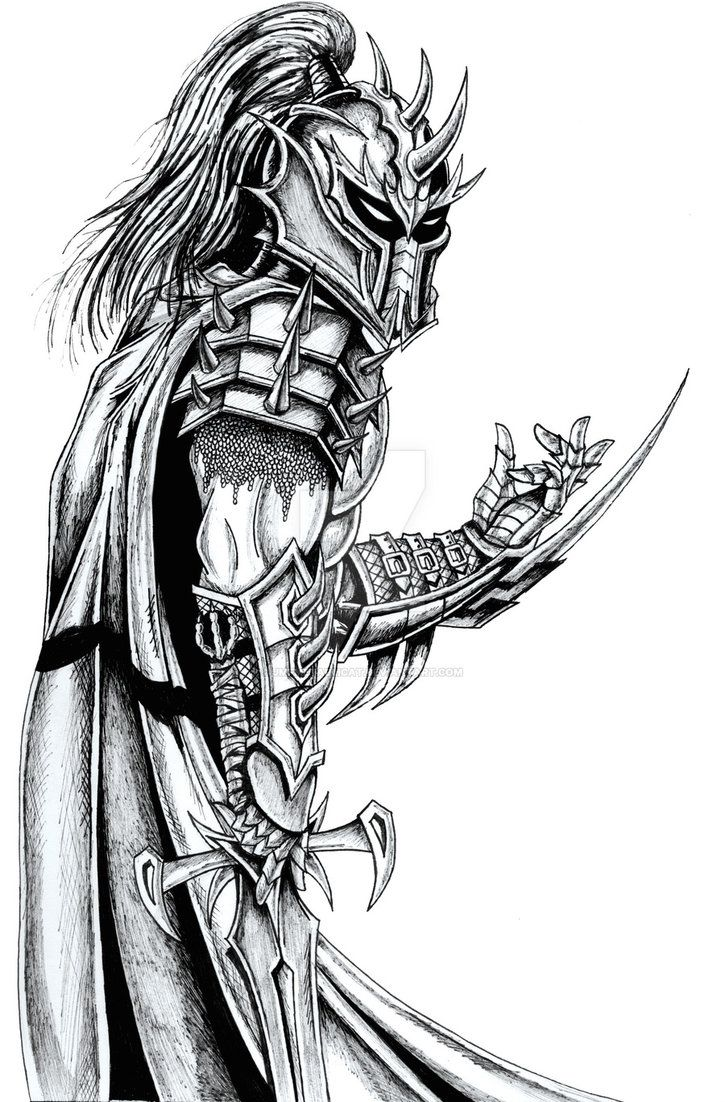
\includegraphics[width=0.7\linewidth,height=\textheight,keepaspectratio,alt={Not
all paladins serve a righteous cause\ldots{}}]{darkKnight.jpg}
\caption{\emph{Not all paladins serve a righteous cause\ldots{}}}
\end{figure}

\onecolumn

\clearpage
\thispagestyle{empty}
\begin{center}
\vspace*{\fill}
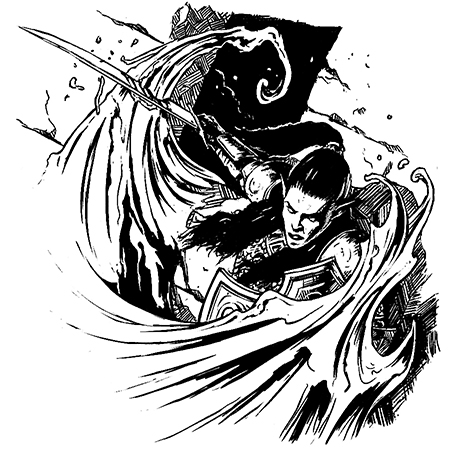
\includegraphics[width=0.7\textwidth,keepaspectratio]{elfPaladin.jpg}\par
\vspace{0.4cm}
{\itshape An elf paladin beats back the forces of darkness.}\par
\vspace*{\fill}
\end{center}

\end{document}